
\subsection{A generic CAP pair}

Consider a general pair of CAP ellipses denoted $\E$ and $\E_c$. We will derive a generic parametrization for the vertices of 3-periodics in such a pair. A first calculation will be helpful. Referring to \cref{fig:ell-ints}(left), the following are coordinates for the intersections $P_2$ and $P_3$ on $\E$ of the two tangents to $\E_c$ seen from a point $P_1=[x_1,y_1]$ also on $\E$:

\begin{figure}
    \centering
    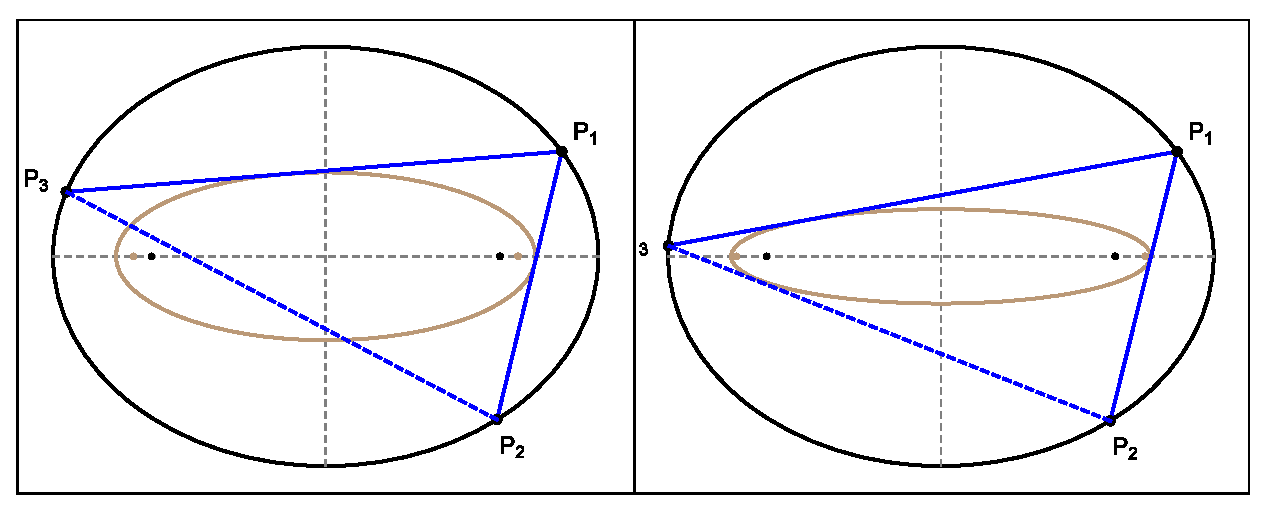
\includegraphics[width=\textwidth]{pics_03_070_ell_ints.eps}
    \caption{\textbf{Left:} Two CAP ellipses (black and brown), and a point $P_1$ on the outer one. The lines thru $P_1$ tangent to the inner ellipse intersect the outer one at $P_2$ and $P_3$. Notice that $P_2 P_3$ cut thru the inner ellipse, i.e., the pair of ellipses does not satisfy Cayley's conditions. \textbf{Right:} the minor axis of the inner ellipse has been scaled such that $P_1 P_2 P_3$ is now a Poncelet triangle.}
    \label{fig:ell-ints}
\end{figure}

\begin{align}
    P_2& =[x_2,y_2]=\frac{1}{k_2}\left[\frac{u_1 x_1 + u_2 y_1}{b} ,  \frac{w_1 x_1 + w_2 y_1}{a} \right] \label{eq:03-n3-conc-general} \\
    P_3&=[x_3,y_3]=\frac{1}{k_2}\left[\frac{w_1 x_1 - w_2 y_1}{b},\frac{w_1 x_1 - w_2 y_1}{a}\right] \nonumber
\end{align}
where:
\begin{align*}
    u_1 &=b\left(a^4  b_c^4 -(a^2 -  a_c^2)^2 b^4 \right) \\
    u_2 &= 2 a k_1 \left( (a^2 + a_c^2)b^2 - b_c^2 a^2\right) \\
    k_1&=\sqrt{ b^2  b_c^2 (a^2 -  a_c^2)  x_1^2 +  a_c^2 a^2(b^2 -  b_c^2)  y_1^2}\\
    k_2 &=\left(\frac{a^2 (b^2 +  b_c^2) - a_c^2 b^2 }{a}x_1\right)^2+ \left(\frac{a^2 (b^2 -  b_c^2) + a_c^2b^2 }{b} y_1\right)^2\\
    w_1&=2 b k_1\left( (b^2 +  b_c^2) a^2 - a_c^2 b^2\right) \\
    w_2&= a\left(a_c^4b^4-a^4(b^2-b_c^2)^2\right)
     %=-a (a^2( b^2 -    b_c^2) -  a_c^2 %b^2) (a^2 (b^2 -   b_c^2) +  a_c^2 b^2)
\end{align*}
 
\subsection{Brocard Porism}

Consider an isosceles Poncelet triangle $\Tm=ABC$ in the Brocard porism, where $AB$ is tangent to $\E$ at one of its minor vertices. Let $|AB|=2d$ and the height be $h$. Let $\zeta=d^2+h^2$. Let the origin $(0,0)$ be at its circumcenter $X_3$. Its vertices will be given by:

\[A=\left[-d ,\frac{d^2-h^2}{2h}\right], \;\;\; B= \left[d,\frac{d^2-h^2}{2h}\right], \;\;\; \left[0 ,\frac{\zeta}{2h}\right] \]


\begin{proposition}\label{prop:pair_brocard}
The Brocard porism containing $\Tm$ as a Poncelet triangle is defined by the following circumcircle $\K_0$ and Brocard inellipse $\E$:

\begin{align*}
\K_0:& x^2+y^2-R^2=0, \;\;\; R=\frac{\zeta}{2h}\\
\E:& -64d^2  h^4  x^2-4  h^2  (9  d^2+h^2)  \zeta  y^2 +4  h  (3  d^2+h^2)  (3  d^2-h^2)  \zeta  y\\&-(d^2-h^2) (9d^2 -h^2) \zeta^2=0
\end{align*}
\end{proposition}

\begin{proof}
The proof follows from $\Tm$, and isosceles Poncelet triangle. Recall that the Brocard inellipse is centered at $X_{39}$. Its perspector is $X_6$, i.e., it will be tangent to $\Tm$ where cevians through $X_6$ intersect it; see \cite[Brocard inellipse]{mw}.
\end{proof}


Consider the pair: circle $x^2+y^2=R^2=(d^2+h^2)^2/(4h^2)$ and   ellipse
$x^2/a^2+(y-y_0)^2/b^2=1$, with  semi-axes
 \[  (a,b)=\left(\frac{d\sqrt{d^2+h^2}}{9d^2+h^2},\frac{4d^2}{9d^2+h^2}\right)
    \]
and center $(0,y_0)$,  $y_0=(9d^4 - h^4)/(2h(9d^2  +  h^3))$.

Vertices $P_i=[x_i,y_i]$, $i=1,2,3$ of Brocard porism triangles are given by:

{\small  
\begin{equation}
    \aligned
    x_1 &= \cos{t}/q_1\\
    y_1 &= \sin{t}/q_1 \\
    x_2 &= -d (d^2 + h^2) ((3 d^2 + h^2)\sin{t} + 2d h \cos{t}- 3 d^2 + h^2)/q_2 \\
    y_2&=-(d^2 + h^2) ((9 d^4 - 2 d^2 h^2 + h^4)\sin{t} - 2 d h (3 d^2 + h^2)\cos{t} - 9 d^4 + h^4)/(2 b q_2) \\
    x_3 &= d (d^2 + h^2) (2 d h \cos{t} - (3 d^2 + h^2) \sin{t} + 3 d^2 - h^2)/q_3\\
    y_3 &=(d^2 + h^2) (2d h (3 d^2 + h^2) \cos{t}+ (9 d^4 - 2 d^2 h^2 + h^4)\sin{t} - 9 d^4 + h^4)/(2 b q_3) \\
    q_1&=(2h)/(d^2+h^2)\\
    q_2&= 2 d h (3 d^2 - h^2)\cos{t} - (9 d^4 - h^4) \sin{t}  + 9 d^4 + 2 d^2 h^2 + h^4\\
    q_3&= 2 d h (3 d^2 - h^2)\cos{t} + (9 d^4 - h^4)\sin{t} - 9 d^4 - 2 d^2 h^2 - h^4
\endaligned
\label{eqn:03-vertices-brocard}
\end{equation}
}
